%start preamble
\documentclass[paper=a4,fontsize=11pt]{scrartcl}%kind of doc, font size, paper size

\usepackage{fontspec}
\defaultfontfeatures{Ligatures=TeX}
%\setsansfont{Liberation Sans}
\usepackage{polyglossia}	
\setdefaultlanguage[spelling=new, babelshorthands=true]{german}
			
\usepackage{amsmath}%get math done
\usepackage{amsthm}%get theorems and proofs done
\usepackage{graphicx}%get pictures & graphics done
\graphicspath{{pictures/}}%folder to stash all kind of pictures etc
\usepackage{amssymb}%symbolics for math
\usepackage{amsfonts}%extra fonts
\usepackage{caption}%captions under everything
\usepackage{listings}
\numberwithin{equation}{section} 
\usepackage{float}%for garphics and how to let them floating around in the doc
\usepackage{xcolor}%nicer colors, here used for links
\usepackage{dsfont}
\usepackage{stmaryrd}
\usepackage{geometry}
\usepackage{hyperref}
\usepackage{fancyhdr}
\usepackage{multicol}
\usepackage{csquotes}
\usepackage{enumitem}

\usepackage[backend=biber,style=alphabetic,
citestyle=alphabetic]{biblatex} %biblatex mit biber laden
\addbibresource{sources.bib}

%settings colors for links
\hypersetup{
    colorlinks,
    linkcolor={blue!50!black},
    citecolor={blue},
    urlcolor={blue!80!black}
}

\definecolor{pblue}{rgb}{0.13,0.13,1}
\definecolor{pgreen}{rgb}{0,0.5,0}
\definecolor{pred}{rgb}{0.9,0,0}
\definecolor{pgrey}{rgb}{0.46,0.45,0.48}

%Header & Footers
\pagestyle{fancy}
\lhead{Netzwerke -- Übung\\Sommersemester 2021}
\rhead{FB 4 -- Angewandte Informatik\\Hochschule für Technik und Wirtschft Berlin}
\lfoot{Übungsblatt 03 -- Routed LAN}
\cfoot{}
\fancyfoot[R]{\thepage}
\renewcommand{\headrulewidth}{0.4pt}
\renewcommand{\footrulewidth}{0.4pt}

\lstdefinestyle{Bash}{
  language=bash,
  showstringspaces=false,
  basicstyle=\small\sffamily,
  numbers=left,
  numberstyle=\tiny,
  numbersep=5pt,
  frame=trlb,
  columns=fullflexible,
  backgroundcolor=\color{gray!20},
  linewidth=0.9\linewidth,
  %xleftmargin=0.5\linewidth
}


%%here begins the actual document%%
\newcommand{\horrule}[1]{\rule{\linewidth}{#1}} % Create horizontal rule command with 1 argument of height

\DeclareMathOperator{\id}{id}

\begin{document}
\begin{center}
\Large{\textbf{Hausaufgaben Laborübung 03 -- Statisches Routing}}
\end{center}
\begin{center}\Large{\textbf{Aufgabe A - Wiederholung Routing}}
\end{center}\vskip0.25in
Nachdem sie im letzten Übungsblatt ihr Netzwerk durch einen Switch (wenn auch nur virtuell) verbunden haben und hierdurch ihre Kommunikation aufbauten, \enquote{wandern} sie im kommenden Übungsblatt im OSI-Modell eine Schicht weiter nach oben.\\
Es soll folglich ein Netzwerk geplant und umgesetzt werden, das auf Routing setzt. Der Router ist fortan zentrale Anlaufstelle für die Kommunikation. Diese Umsetzung hat den Vorteil, dass der Router Pakete über Netzgrenzen hinweg vermitteln kann. Ihr kleines, abgeschottetes Netzwerk kann über die bisherigen Grenzen hinweg kommunizieren.
\begin{enumerate}
	\item Als Wiederholung des Vorlesungsstoffs können sie folgenden Kapitel lesen: \cite[Kap. 4.1, 4.3]{Kurose2012}
	\item Was sind die Aufgaben eines Routers. Wie erfolgt, im Groben, die Umsetzung des Routings?
	\item Nennen sie einige Routing-Protokolle. Ist ihnen eines (oder mehrere) dieser Protokolle bereits begegnet?
	\item Machen sie sich klar, wie Router und IP-Protokoll zusammenhängen.
	\item In welche Schicht des OSI-Modells würden sie einen Router einordnen? (Begründung!)
	\item Wie haben sich bis jetzt ihre VMs gefunden? Woher \enquote{wussten} sie, an welches Gerät die Ethernet-Frames zu schicken waren? Wie spielt hier Ihre eigene IP-Adresse, Ihre Subnetzmaske mit hinein? Bzw. spielt diese auf Hardwareebene eine Rolle?
	\item Woher weiß ein Rechner, wann er ein Paket direkt adressieren kann und wann er es an Router/Gateway weiterschicken muss?
	\item Woher weiß ein Router, wann er ein Paket weiterschicken soll und wann nicht?
\end{enumerate}


\begin{center}
\Large{\textbf{Aufgabe B -- Planung des Routing zwischen Netzen}}
\end{center}
\vskip0.25in
Im vorigen Aufgabenblatt haben sie zu den IP-Adressen auch eine Netzwerkmaske konfiguriert. Diese Netzwerkmaske legt fest, welche Rechner im gleichen (Sub-)Netz liegen und somit direkt angesprochen werden können. Daraus folgt aber auch, dass bestimmte Rechner außerhalb ihres Netzes nicht direkt angesprochen werden können. Diese können via Router/Gateway erreicht werden.\\
Wir wollen in einem ersten Schritt selber einen Router betreiben, um über unsere kleinen Netze hinweg zu kommunizieren. Dazu erweitern sie ihr Wissen aus dem vorigen Übungsblatt, sodass ihr Netzwerk \enquote{wachsen} kann.
\begin{enumerate}
	\item Erläutern sie was klassenbasierte IPv4-Adressen sind. Wie sind diese Klassen definiert? Woran kann die Klassenzuordnung auf Bitebene festgemacht werden?
	\item Früher wurden Klassen von Adressen genutzt, heute das nutzt man \emph{CIDR (Classles Inter Domain Routing)}. Worin unterscheiden sich \emph{CIDR} und klassenbasierten Adressen?
	\item Recherchieren sie, warum sich dies änderte!
	\item Recherchieren sie wie die Syntax der klassenbasierten Notation aussieht und geben sie einige Beispiele für die Notation.
	\item Recherchieren sie wie die Syntax der \emph{CIDR}-Notation aussieht und geben sie einige Beispiele für die Notation.
	\item In der kommenden Übung soll ihr konfiguriertes Netzwerk umgebaut werden. Aus einem Netzwerk sollen zwei werden.\\
	Um zwischen den beiden lokalen Netzwerken kommunizieren zu können, benötigen sie einen Router. Eine VM soll diese Aufgabe übernehmen. Der Router muss so konfiguriert werden, dass klar ist wohin die Pakete geschickt werden. Das heißt: Pakete die nicht in das eigene, lokale Netzwerk gehören, werden über den Router in die externen Netzwerke weitergereicht.
	\begin{figure}[h]
	\centering
	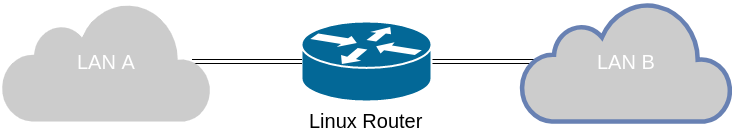
\includegraphics[scale=0.35]{lan}
	\caption{Skizze des Netzwerkes bestehend aus zwei LANs und einem Router. Ignorieren sie das dort noch Linux-Router steht!}
	\end{figure}
	\begin{enumerate}
		\item Unterteilen sie ihr Netzwerk, sodass sich im Idealfall zwei VMs in einen lokalen Netzwerk $A$ und zwei VMs im lokalen Netzwerk $B$ befinden. Zwischen beiden Netzen vermittelt ein Router. Falls ihre Rechenressourcen nicht ausreichen, sind auch drei Rechner für die praktische Umsetzung ausreichend.
		\item Skizzieren sie ihre lokalen Netzwerke, sowie das gesamte Netzwerk (D.h. nutzen sie geeignete Symbole s. letztes Übungsblatt).
		\item Wir nutzen für die Umsetzung private IPv4-Adressen. Welche IPv4-Adressen stehen ihnen für die Umsetzung des Netzwerkes zu Verfügung? Wählen sie eine IPv4 und IPv6 Range, die für die Umsetzung geeignet ist.
		\item Vergeben sie entsprechende IPv4-Adressen mit kleinst mögliche Subnetzmasken auf der Skizze. Vergeben sie ebenso IPv6-Adressen. Gilt für IPv6 die gleiche Voraussetzung bezüglich der Netzgröße?
		\item Planen sie ebenso den Router mit entsprechenden IP-Adressen auf der Skizze ein. Achten sie darauf, dass der Router als Verbindungsstück (Intermediate-Node/Zwischenknoten) zwischen Ihren beiden Netzen fungiert und dementsprechend beide Netzwerke kennen muss. Das heißt, der Router muss mindestens zwei IP-Adressen haben, jeweils eine pro Netzwerk. Möglicherweise hat ihr Router auch zusätzliche Adapter und Adressen, beispielsweise für den Uplink ins Internet.
	\end{enumerate}
\end{enumerate}

\begin{center}
\Large{\textbf{Aufgabe C -- NAT}}
\end{center}
\vskip0.25in

In der Vorlesung haben sie zunächst den allgemein Aufbau von IP-Adressen besprochen. Auch das es private IP-Adressbereiche gibt. Diese wurden aus den Gesamtraum der IP-Adressen gelöst, um für den privaten Gebrauch verfügbar zu sein. D.h. diese Adressen können nicht geroutet werden. Da unsere VMs jedoch auch mit dem Internet kommunizieren können sollen benötigen wir noch eine weitere Technologie -- \emph{NAT}. Mithilfe von \emph{NAT} (Network Address Translation) können private IPv4-Adressen auf global routbare Adressen abgebildet werden.

\begin{enumerate}
	\item Lesen sie \cite[S. 349ff]{Kurose2012} oder \cite{fall2011tcp} als Einführung zum Thema \emph{NAT}. Ihnen sollte klar sein, welche Aufgabe \emph{NAT} erledigt und wie \emph{NAT} im Groben umgesetzt wird.
	\item Unser Router bekommt eine zusätzliche Funktion, er wird ein \emph{NAT}-Gateway -- genau gesagt ein \emph{PAT}-Gateway. Recherchieren sie, was unter Port Address Translation verstanden wird. Wo liegt der wesentliche Unterschied zum gewöhnlichem \emph{NAT}?
	\item Erklären sie was ein \emph{NAT}-Table ist. Was wird in dieser Tabelle hinterlegt? Was wird hier beim \emph{PAT} hinterlegt?
	\item Erklären sie ganz grob die Idee einer Firewall.
	\item Lesen sie folgenden Eintrag im \emph{freeBSD}-Handbuch: \url{https://www.freebsd.org/doc/de_DE.ISO8859-1/books/handbook/firewalls-pf.html}. Dieser Eintrag hilft ihnen bei der Umsetzung des \emph{NAT}s.
\end{enumerate}


\begin{center}
\Large{\textbf{Aufgabe D -- Tools \& OS}}
\end{center}
\vskip0.25in

\begin{enumerate}
	\item Seit der letzten Übung kennen sie einige grundlegende Befehle, um das Netzwerkinterface eines unixoiden Betriebssystems zu konfigurieren. Dieses Wissen soll nun erweitert werden. Hierfür schauen wir in die bekannten Werkzeugkästen \emph{iproute2} und \emph{net-tools}.
	\begin{enumerate}
	\item Recherchieren sie, welches Tool aus \emph{iproute2} genutzt werden kann um Routen zu setzen. Notieren sie sich die Syntax und was die Parameter bewerkstelligen.
	\item Analog dazu: Wie werden Routen mithilfe der \emph{net-tools} konfiguriert?
	\item \url{https://www.freebsd.org/doc/de_DE.ISO8859-1/books/handbook/network-routing.html} bietet ihnen eine gute Anlaufstelle, wie Router und Routing unter \emph{freeBSD} umgesetzt wird.
	\item Recherchieren sie beispielhaft wie eine persistente Lösung aussähe.\footnote{Persistent heißt in diesem Kontext, wie die Konfiguration dauerhaft im Betriebssystem festgehalten wird -- im wesentlich in welche Konfigurationsdateien muss geschrieben werden.}\\
	Kommentieren sie ihr Beispiel anschließend, sodass sie wissen was die einzelnen Zeilen bedeuten.
	\end{enumerate}
	\item Gateways \& Router -- Gateways sind im allgemeinen nicht das Gleiche wie Router. Auch unter den Gateways gibt es Unterscheidungen.
	\begin{enumerate}
	\item Recherchieren sie worin sich Router und Gateways unterscheiden.
	\item Beim aufsetzen des Netzwerkes kann unterschieden werden zwischen \emph{Gateways} und \emph{Default Gateways}. Recherchieren sie diese Unterscheidung.
	\end{enumerate}
	\item Im vorigen Übungsblatt arbeitete ihr Netzwerk mithilfe eines Switches. Alle Knoten des Netzwerkes waren innerhalb eines Segments (LAN). Daher konnte sie nur innerhalb Ihres Netzwerkes kommunizieren, darüber hinaus aber nicht. Mithilfe eines Routers erweitern sie die Reichweite ihres Netzwerkes. Jedoch ist Routing ein wesentlich komplexerer Vorgang, da in der Regel Wege zwischen Endknoten durch ein Netzwerk gefunden werden müssen (Route). Aufgrund dieser Tatsache müssen sie ein wenig tiefer in das Betriebssystem schauen.
	\begin{enumerate}
	\item Recherchieren sie mit den vorangegangen Quellen, was ein Routing-Table/Routing-Tabelle ist \footnote{\url{https://docs.freebsd.org/doc/12.1-RELEASE/usr/local/share/doc/freebsd/de_DE.ISO8859-1/books/handbook/network-routing.html}}.
	\item Recherchieren sie den Unterschied zwischen Forwarding und Routing.
	\item Wie aktivieren sie unter \emph{freeBSD} das Forwarding? Analog: Wie wird  das Forwarding unter Linux (Arch-Linux) eingeschaltet?
	\item In welcher Konfigurationsdatei müssen sie einen Eintrag vornehmen, so das das Routing dauerhaft beim Systemstart aktiviert bleibt? Notieren sie sich beispielhaft (auszugsweise) wie dies aussehen kann.
	\end{enumerate}
	\item Das Internet Control Message Protocol (ICMP) wird in Netzwerken als Diagnosetool zum Austausch von Informations- und Fehlermeldungen verwendet. 
	\begin{enumerate}
		\item \textbf{Wiederholung:} Recherchieren sie welchen Hinweis Ihnen dabei die verschiedenen ICMP-Fehlermeldungen geben -- wo wird jeweils der Fehler in der Konfiguration liegen?
		\begin{enumerate}
			\item Connect: network is unreachable
			\item Destination Host Unreachable
			\item Destination Network Unreachable
			\item Keine Antwort auf ein Ping
		\end{enumerate}  
	\end{enumerate}
\end{enumerate}

\begin{center}
\Large{\textbf{Aufgabe E -- Vorbereitung Laborübung}}
\end{center}
\vskip0.25in
\begin{enumerate}
	\item Importieren und klonen sie die benötigten VMs!
	\begin{enumerate}
		\item Optimal: Zwei Netzwerke mit je einer \emph{freeBSD}- und einer Linux-VM. (Falls Ressourcen knapp sind, zwei Netzwerke mit einem \emph{freeBSD} und einem Linux). Nutzen sie die VMs ohne grafische Oberfläche! Bei Bedarf können sie die Ressourcen der VMs weiter herunter- oder heraufsetzen.
		\item Als Router soll das \emph{freeBSD} mit grafischer Oberfläche zum Einsatz kommen.
		\item Konfigurieren sie die Adapter, sodass ihre VMs in den entsprechenden virtuellen Netzwerken arbeiten (Host-Only Network)
		\begin{enumerate}
			\item Tutorial Import unter virtualBox im Moodle
			\item Tutorial Einstellen der Netzwerkadapter im Moodle
			\begin{itemize}
				\item Die VMs die nur Hosts sind haben einen aktiven Adapter für ein Host-Only-Network.
				\item Der Router hat drei aktive Adapter, ein Bridge und zwei Host-Only-Network.Adapter.
			\end{itemize}
		\end{enumerate}
		\item Konfigurieren sie den \emph{freeBSD}-Router. Diese VM hat drei aktive Adapter: 
		\begin{itemize}
			\item Bridge-Mode
			\item Host-Only Network $A$
			\item Host-Only Network $B$
		\end{itemize}
	\end{enumerate}
	\item Lesen sie vorbereitend das Laborübungsblatt! Notieren sie sich bei allen Aufgaben, die ihnen nicht klar sind ihre Fragen. 
	\item Notieren sie sich alle Fragen zu Aufgaben, bei denen sie kein Lösungsansatz haben.
\end{enumerate}

\printbibliography
\end{document}
